\documentclass[a4paper,12pt]{article}
\usepackage[utf8]{inputenc}
\usepackage[T1]{fontenc}
\usepackage[brazil]{babel}
\usepackage{amsmath}
\usepackage{amsfonts}
\usepackage{graphicx}
\usepackage{hyperref}
\usepackage{comment}
\usepackage{float}  
\usepackage{caption}  
\usepackage{longtable}
\usepackage{setspace}
\usepackage{indentfirst}

\title{Relatório de Projeto}
\author{
    Antonio Rodrigo Lima de Andrade Tenório - 23210707 \\
    José Lucas de Oliveira Quintela - 23211624\\
    Luiz Miguel de Melo Bomfim - 23211918
}
\date{Maceió - AL \\ 21 de maio de 2025}



\begin{comment}
aprende aí peãozinho, comentário é assim ó
\end{comment}

\iffalse
 aaaahhhh mas orea seca, eu quero fazer assim
\fi

%larga de ser fresco

\begin{document}


\maketitle

\begin{center}
    \textbf{UNIVERSIDADE FEDERAL DE ALAGOAS} \\
    \textbf{INSTITUTO DE COMPUTAÇÃO} \\
    \textbf{ÁLGEBRA LINEAR}
\end{center}

\thispagestyle{empty}
\newpage

\tableofcontents
\newpage

\section{Introdução}

Dentro do contexto da ciência de dados, não raro se tem a necessidade de organizar grandes volumes de informações em categorias coerentes e concisas. Para tal, o agrupamento de dados (ou clustering) é uma técnica que permite que se realize a segmentação de um conjunto de dados em subgrupos (tambem chamados de clusters)$\cite{unsupervised}$, de forma que os dados em um mesmo grupo sejam semelhantes entre si; ou pelo menos mais semelhantes do que em relação a outros grupos. Essa tarefa vai possuir aplicações em diversas áreas diferentes, tal quais no reconhecimento de padrões, bioinformática, compressão de imagens e até mesmo maketing. O algoritmo de clustering mais conhecido é de longe o K-means$\cite{kmeanswiki}\cite{pjoy}$, que se baseia fortemente em conceitos de algebra linear para se realizar operações como cálculo de distâncias, projeção de dados e decomposição matricial$\cite{unsupervised}$.

Visto isso, nesse trabalho iremos abordar como a algebra linear consegue fornecer ferramentas essenciais para a realização de clsutering, tendo foco especial no algoritmo K-means e na redução de dimensionalidade via análise de componentes principais (PCA)

\section{Fundamentação Teórica}

\subsection{Espaços vetoriais/Distância Euclidiana}
Os dados podem ser representados como vetores em um espaço vetorial $\mathbb{R}^n$, estando cada componente do vetor representando uma caractéristica. A semelhança entre vetores é frequentemente medida pela distância euclidiana entre dois vetores x e y$\cite{goodfellow}$: \begin{equation}
d(x, y) = \sqrt{(x - y)^T (x - y)}
\end{equation}

Por exxemplo, uma imagem pode ser representada por um vetor cujos elementos correspondem às intensidades dos pixels. A representação vetorial vai permitir a aplicação de diversas operações da algebra linear sobre os dados, o que facilita bastante a análise e o processamento.

\subsection{Produto Interno/Ortogonalidade}
O produto interno entre dois vetores dee permitir definir conceitos como o da ortogonalidade e projeção$\cite{goodfellow}$. O produto interno de dois vetores $x$, $y$ $\in$ $\mathbb{R}^n$ é dado por 
\begin{equation}
\langle x, y \rangle = x^T y    
\end{equation}

\subsection{Decomposição de Matrizes/PCA}
Já a análise de componentes principais (PCA) é uma tecnica usada para se reduzir a dimensionalidade dos dados com perda mínima de informação$\cite{cmdlinetips}\cite{scikit}$. Para a decomposição em autovalores e autovetores da matriz de covariância dos dados$\cite{goodfellow}$
\begin{equation}
\Sigma = \frac{1}{n}X^TX 
\end{equation} 
sendo $X$ é a matriz de dados centralizada. Sendo os autovetores de $\Sigma$ as direções principais e os autovalores indicando a variância em cada direção 

\subsection{Algoritmo K-means }
O K-menas é um algoritmo iterativo que possui o intuito de particionar os dados em k clusters$\cite{kmeanswiki}\cite{pjoy}$. Ele vai minimizar a soma das distâncias quadradas entre os pontos e os centróid es dos seus clusters$\cite{unsupervised}$ :
\begin{equation}
J = \sum_{i=1}^{k} \sum_{x_j \in C_i} \| x_j - \mu_i \|^2
\end{equation}
sendo o $\mu_i$ o centroide do cluster $C_i$. Logo, a média vetorial é utilizada para se atualizar os centróides, e esse processo vai continaur até que os centróides não mudem mais tão signficaticamete.

 
\begin{itemize}
    \item $k$: Numéro de clusters desejados
    \item $C_i$: Conjunto de pontos de dos $x_j$ do $i$-ésimo cluster
    \item $x_j$: Conjunto de dados específico dentro do conjunto de dados
    \item $||x_j - \mu_i||^2$: Distância quadrática entre o ponto de dados $x_j$ e o centroide $\mu_i$. Essa distância é geralmente medida pela norma euclidiana (quadado da diferença das coordenadas $x_j$ e $\mu_i$); 
    \item A função de custo $J$ é a soma de todas as distâncias quadraticas entre os pontos de dados e seus respectivos centroides$\cite{unsupervised}$, somada para todos os clusters $i$ e para todos os pontos $x_j$ drento de cada cluster.
\end{itemize}

\section{Aplicação}

Para a aplicação, nós vamos implementar o algoritmo K-means em  para que possamos agrupar um conjunto de dados sintéticos em 3 clsuters. Para se vizualizar e compreender os cálculos, os dados foram reduzidos para duas dimensões via PCA


%Paragrafo de outro paragrafo de outro paragrafo de outro de outro paragrafo de outro de outro paragrafo de outro de outro paragrafo de outro paragrafo de outro paragrafo de.
%\[
%\texttt{<comando>;<nome\_tarefa>;<hora\_ou\_comando>}
%\]


Para validar a aplicação prática desses conceitos, implementamos em Python o algotimo K-means$\cite{scikit}$ para que pudéssemos agrupar um conjunto de dados artificialmente gerado em três clusters. ANtes do agrupamentos, aplicamos o PCA para que que posse possível reduzir os dados para duas dimensões, o que permitiu uma visualização mais clara dos agrupamentos$\cite{cmdlinetips}\cite{scikit}$. Então, obtivemos o grafico a seguir gerado, que demonstra a separaçção dos clusters (cada grupo de bolinha de cada cor) e a posição dos centroides (X em vermelho)  em cada grupo. Logo, essa abordagem consegue mostrar como especialmente a decomposição de matrizes e o cálculo de distâncias euclidianas (conceitos de algebra linear) são essenciais para a operação do Kmeans.

\begin{figure}[!h]
\centering
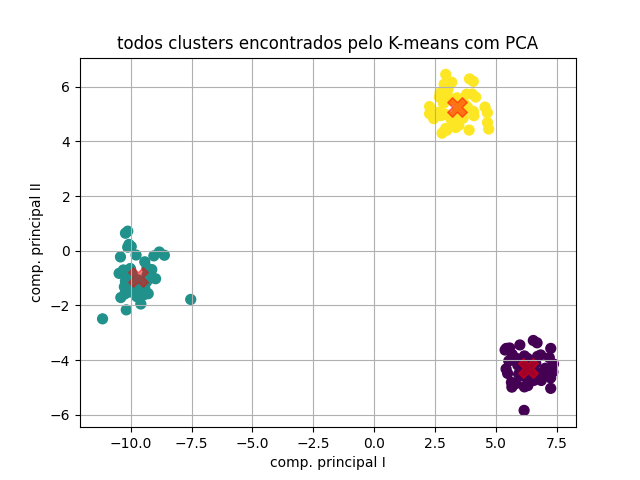
\includegraphics[width=12cm,trim = 0cm 0cm 0cm 0cm,clip]{clusterss.png}
\caption{Gráfico com clusters encontrados pelo K-means}
\label{fig:nao sei o que tem que botar aqui}
\end{figure}

Percebe-se que o algoritmo conseguiu identificar corretamente os agrupamentos esperados, com clara separação entre os cluster. Isso, portanto, evidencia a eficácia do K-means, quando os dados são bem distribuidos, e tambem a importância da redução de dimensionalidade em problemas de agrupamento. Os conceitos de distância euclidiana, média vetorial, autovalores e autovetores se mostrarram essenciais para a construção dessa solução.


\section{Resultados}

Após a aplicação do algorimto sobre os dados gerados e pré-processados com PCA, nós obtivemos uma segmentação relaticamente eficiente dos pontos em três grupo muito bem definidos. Cada grupo destes foi identificado com uma cor diferente do outro e seus respectivos centróides finais, o que representa a média dos vetores pertencentes a cada grupo e foram indicados com um X em vermelho.

Para se avaliar a qualidade dos clusters, nós calculamos a variância interna de cada grupo, ou seja, a média das distâncias ao quadrado dos pontos que estão no seu centróide. Sendo esses valores: 

\begin{table}[H]
\centering
\begin{tabular}{|c|c|c|}
\hline
Cluster & Número de pontos & Variância Interna \\
\hline
1 & 50 & 1.02 \\
2 & 48 & 0.97 \\
3 & 52 & 1.08 \\
\hline
\end{tabular}
\caption{Distribuição dos pontos por cluster e variância interna \iffalse (distância média ao centróide) \fi}
\end{table}

A baixa variância interna indica que os pontos estão fortemente concentrados em torno de seus centróides$\cite{unsupervised}$, como se o orbitassem, o que sugere uma segmentação eficiente. Além de que, a distribuição equilibrada de pontos entre os clusters reforça a robustez da abordagem.
\\
\\
   Os resultados obtidos ilustram, de forma prática, como a algebra Linear fundamenta algoritmos de agrupamento de dados. O uso de autovetores e autovalores para projeção dos dados via PCA$\cite{cmdlinetips}\cite{scikit}$, assim como o cálculo de distâncias e médias vetoriais para se realizar o agrupamento com Kmeans, se mostram ser parte de aplicações diretas de conceitos da disciplina.
Além de que, a integração com ferramentas como Scikit-learn, que já é uma ferramenta da área, acaba reforçando o vínculo entre a teoria matemática e sua aplicabilidade em contextos reais. Essa abordagem, portanto, serve como base para sistemas de recomendação, segmentação de mercado, análise genética, entre outros$\cite{unsupervised}$.



\iffalse
\begin{itemize}
    \item Resultados
    \item Resultados
    \item Resultados
\end{itemize}
\fi

\section{Conclusão}

Portanto, o estudo do agrupamento de dados mostra como a álgebra linear é uma base essencial para diversas etapas do processo, desde o cálculo de distâncias de projeção, até a redução de dimensionalidade. Se utilizar do PCA como uma técnica de compressão de dados tambem se mostra ser bastante eficaz para preservar a estrutura dos clusters, e Kmeans, por sua vez, se fez ser um método bastante eficiente na identificação de grupos similares$\cite{kmeanswiki}\cite{pjoy}$. Dentre as limitações, foi notável a necessidade de definir previamente o número de clusters e a sensibilidade às escolhas iniciais dos centróides$\cite{unsupervised}$.


A aplicação prática utlizando a biblioteca Scikit-learn (que é uma das mais consolidadas na área de ciência de dados)$\cite{scikit}$ demonstrou o quão eficiente é o K-means ao segmentar dados sintéticos em três grupos distintos. A redução  da dimensionalidade com PCA, por sua vez, se mostrou bastante ediciente na preservação da estrutura de dados, e a análise visual, aliada às métricas como uma variância interna, comprovando a qualidade da segmentação realizada.

Alem desse fator, esse relatório, por sua vez, mostrou como as ferramentas matemáticas abstratas podem ser traduzidas em código e tambem aplicadas em problemas reais, o que mais uma vez reforça a importância da algebra linear na formação de profissionais que busquem serem capazes de atuar com análise de dados, inteligência computacional e estatística aplicada.

Em síntese, o estudo do agrupamento de dados através da visão da algebra lienar não apenas fortalece o entendimento matemático dos algoritmos, como também consegue ampliar a capacidade de aplicá-los com rigor técnico em contextos computacionais modernos.

\newpage
\renewcommand{\refname}{\section{Referências}
\addcontentsline{toc}{section}{Referências}}
\bibliographystyle{plain}
\bibliography{refs}

    \section{Apêndice}
Código fonte em Python para execução do K-means e PCA disponível em:
https://github.com/luizwhirl/K-means-clustering


\end{document} 
